
\NeedsTeXFormat{LaTeX2e}
\LoadClass{article}
\RequirePackage{todonotes}
\RequirePackage[parfill]{parskip}
\RequirePackage[margin=2.8cm]{geometry}
\RequirePackage{hyperref}
\RequirePackage[english]{babel}
\RequirePackage{pgfplots}
\RequirePackage{listings}
\RequirePackage{amsfonts}
\RequirePackage{subfiles}
\RequirePackage{mathtools}
\RequirePackage[noabbrev,capitalize,nameinlink]{cleveref}

\providecommand{\tightlist}{%
  \setlength{\itemsep}{0pt}\setlength{\parskip}{0pt}}

\begin{document}
\title{\textbf{NI-KOP~--~Task 2}\\
    Optimisation version of the 0/1 knapsack problem}
\author{Daniel Hampl (hampldan)}
\date{\today}
\maketitle

\tableofcontents
\newpage

\section{Introduction}
The knapsack problem is one of the most widespread NP-Complete problems. It can be described as having a knapsack with a limited capacity and multiple items, where each of these items has a set value and weight. Our task is to fill the knapsack with items of highest combined value possible.

In this paper, we will be focussing approximation algorithms solving the knapsack problem and the deviation of results provided by these approximation algorithms.

\subsection{Definition\cite{WEBSITE:knapsackDef}}
We have weight $W$ and $n$ items, where item $i$ is described as a pair $(w_i, v_i)$.

\begin{itemize}
    \item $w_i$ is a weight of object $n_i$
    \item $v_i$ is a value of object $n_i$
    \item $w_i, v_i \in \mathbb{N}\setminus\{0\}$
\end{itemize}

Find value $V$, where:

\begin{itemize}
    \item $\sum_i(x_i*v_i) = V$
    \item $\sum_i(x_i*w_i) \leq W$
    \item $x_i \in \{0,1\} \forall i$
\end{itemize}

\subsection{Task}
Implement solution for the optimisation version of the knapsack problem in four versions.

\begin{itemize}
    \item Dynamic programing with decomposition by value or weight
    \item Simple greedy heuristic approximation
    \item Modification of this greedy heuristics, where only the single most valuable item is selected
    \item FPTAS algorithm
\end{itemize}

Experimentally evaluate the dependence of computational complexity on instance size. And deviation of results provided by approximation algorithms as compared to the exact results. 

\begin{figure}
	\centering
	\pgfplotsset{every axis legend/.append style={
		at={(1.05,0.5)},
		anchor=west}}
	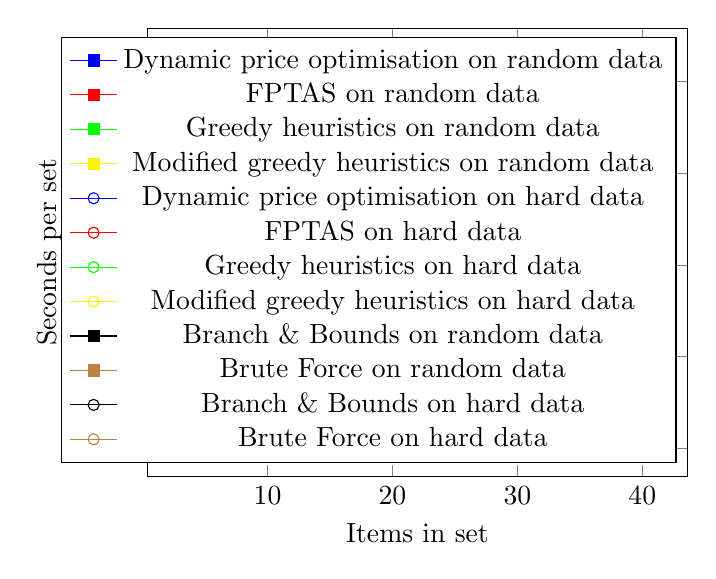
\begin{tikzpicture}
		\begin{semilogyaxis}[
			xlabel=Items in set,
			ylabel=Seconds per set,
			scatter/classes={
				dynN={mark=square*,blue},
				fptasN={mark=square*,red},
				singleN={mark=square*,green},
				hungryN={mark=square*,yellow},
				dynH={mark=o,blue},
				fptasH={mark=o,red},
				singleH={mark=o,green},
				hungryH={mark=o,yellow},
				NSm={mark=square*,black},
				NSt={mark=square*,brown},
				ZSm={mark=o,draw=black},
				ZSt={mark=o,draw=brown}
				}
			]
			\addplot[scatter,%
				scatter src=explicit symbolic]%
			table[meta=label] {
				x y label
				4 .000012 dynN
				10 .000514 dynN
				15 .014872 dynN
				20 .078888 dynN
				22 .114784 dynN
				25 .208052 dynN
				27 .223608 dynN
				30 .291732 dynN
				32 .348044 dynN
				35 .434604 dynN
				37 .547092 dynN
				40 .704324 dynN
			};
			\addplot[scatter,%
				scatter src=explicit symbolic]%
			table[meta=label] {
				x y label
				4 .000010 fptasN
				10 .000144 fptasN
				15 .000690 fptasN
				20 .001822 fptasN
				22 .002398 fptasN
				25 .003606 fptasN
				27 .004508 fptasN
				30 .006790 fptasN
				32 .008502 fptasN
				35 .011454 fptasN
				37 .013754 fptasN
				40 .017528 fptasN
			};
			\addplot[scatter,%
				scatter src=explicit symbolic]%
			table[meta=label] {
				x y label
				4 .000002 hungryN
				10 .000004 hungryN
				15 .000008 hungryN
				20 .000010 hungryN
				22 .000010 hungryN
				25 .000012 hungryN
				27 .000012 hungryN
				30 .000010 hungryN
				32 .000012 hungryN
				35 .000012 hungryN
				37 .000012 hungryN
				40 .000014 hungryN
			};
			\addplot[scatter,%
				scatter src=explicit symbolic]%
			table[meta=label] {
				x y label
				4 .000004 singleN
				10 .000004 singleN
				15 .000010 singleN
				20 .000012 singleN
				22 .000012 singleN
				25 .000012 singleN
				27 .000014 singleN
				30 .000016 singleN
				32 .000016 singleN
				35 .000016 singleN
				37 .000018 singleN
				40 .000020 singleN
			};
			\addplot[scatter,%
				scatter src=explicit symbolic]%
			table[meta=label] {
				x y label
				4 .000010 dynH
				10 .000504 dynH
				15 .014208 dynH
				20 .080942 dynH
				22 .120590 dynH
				25 .204710 dynH
				27 .249138 dynH
				30 .349580 dynH
				32 .435896 dynH
				35 .558234 dynH
				37 .649110 dynH
				40 .792216 dynH
			};
			\addplot[scatter,%
				scatter src=explicit symbolic]%
			table[meta=label] {
				x y label
				4 .000010 fptasH
				10 .000160 fptasH
				15 .000668 fptasH
				20 .001884 fptasH
				22 .002534 fptasH
				25 .004014 fptasH
				27 .005196 fptasH
				30 .007330 fptasH
				32 .009300 fptasH
				35 .012524 fptasH
				37 .014686 fptasH
				40 .019922 fptasH
			};
			\addplot[scatter,%
				scatter src=explicit symbolic]%
			table[meta=label] {
				x y label
				4 .000002 hungryH
				10 .000004 hungryH
				15 .000008 hungryH
				20 .000010 hungryH
				22 .000010 hungryH
				25 .000012 hungryH
				27 .000012 hungryH
				30 .000016 hungryH
				32 .000012 hungryH
				35 .000014 hungryH
				37 .000016 hungryH
				40 .000016 hungryH
			};
			\addplot[scatter,%
				scatter src=explicit symbolic]%
			table[meta=label] {
				x y label
				4 .000002 singleH
				10 .000006 singleH
				15 .000010 singleH
				20 .000014 singleH
				22 .000014 singleH
				25 .000014 singleH
				27 .000016 singleH
				30 .000016 singleH
				32 .000018 singleH
				35 .000018 singleH
				37 .000020 singleH
				40 .000022 singleH

			};
			\addplot[scatter,%
				scatter src=explicit symbolic]%
			table[meta=label] {
				x y label
				4 23.71 NSt
				10 1258.43 NSt
				15 36477.82 NSt
				20 1139944.81 NSt
			};
			\addplot[scatter,%
				scatter src=explicit symbolic]%
			table[meta=label] {
				x y label
				4 7.88 NSm
				10 29.96 NSm
				15 122.98 NSm
				20 637.70 NSm
				22 1718.99 NSm
				25 7495.38 NSm
				27 11446.80 NSm
				30 39577.47 NSm
				32 145111.69 NSm
				35 320850.22 NSm
				37 782664.08 NSm
				40 3304721.06 NSm
			};
			\addplot[scatter,%
				scatter src=explicit symbolic]%
			table[meta=label] {
				x y label
				4 23.70 ZSt
				10 1125.09 ZSt
				15 33469.84 ZSt
				20 1054059.56 ZSt
			};
			\addplot[scatter,%
				scatter src=explicit symbolic]%
			table[meta=label] {
				x y label
				4 14.75 ZSm
				10 324.50 ZSm
				15 5685.97 ZSm
				20 115219.09 ZSm
				22 358548.04 ZSm
				25 2238413.90 ZSm
			};
			\addlegendentry{Dynamic price optimisation on random data}
			\addlegendentry{FPTAS on random data}
			\addlegendentry{Greedy heuristics on random data}
			\addlegendentry{Modified greedy heuristics on random data}
			\addlegendentry{Dynamic price optimisation on hard data}
			\addlegendentry{FPTAS on hard data}
			\addlegendentry{Greedy heuristics on hard data}
			\addlegendentry{Modified greedy heuristics on hard data}
			\addlegendentry{Branch \& Bounds on random data}
			\addlegendentry{Brute Force on random data}
			\addlegendentry{Branch \& Bounds on hard data}
			\addlegendentry{Brute Force on hard data}
		\end{semilogyaxis}
	\end{tikzpicture}
\caption{Time needed depending on number of items in set}
\label{plot:fullTime}
\end{figure}


% \begin{figure}
	\centering
	\pgfplotsset{every axis legend/.append style={
		at={(1.05,0.5)},
		anchor=west}}
	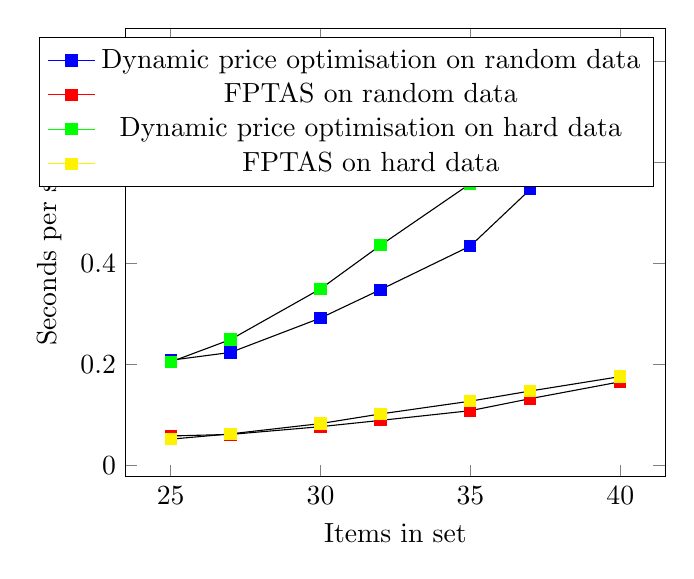
\begin{tikzpicture}
		\begin{axis}[
			xlabel=Items in set,
			ylabel=Seconds per set,
			scatter/classes={
				dynN={mark=square*,blue},
				fptasN={mark=square*,red},
				dynH={mark=square*,green},
				fptasH={mark=square*,yellow}
				}
			]
			\addplot[scatter,%
				scatter src=explicit symbolic]%
			table[meta=label] {
				x y label
				25 .208052 dynN
				27 .223608 dynN
				30 .291732 dynN
				32 .348044 dynN
				35 .434604 dynN
				37 .547092 dynN
				40 .704324 dynN
			};
			\addplot[scatter,%
				scatter src=explicit symbolic]%
			table[meta=label] {
				x y label
				25 .057974 fptasN
				27 .061048 fptasN
				30 .076414 fptasN
				32 .088828 fptasN
				35 .108118 fptasN
				37 .132000 fptasN
				40 .165394 fptasN
			};
			\addplot[scatter,%
				scatter src=explicit symbolic]%
			table[meta=label] {
				x y label
				25 .204710 dynH
				27 .249138 dynH
				30 .349580 dynH
				32 .435896 dynH
				35 .558234 dynH
				37 .649110 dynH
				40 .792216 dynH
			};
			\addplot[scatter,%
				scatter src=explicit symbolic]%
			table[meta=label] {
				x y label
				25 .051640 fptasH
				27 .062136 fptasH
				30 .082542 fptasH
				32 .101642 fptasH
				35 .126996 fptasH
				37 .147170 fptasH
				40 .175732 fptasH
			};
			\addlegendentry{Dynamic price optimisation on random data}
			\addlegendentry{FPTAS on random data}
			\addlegendentry{Dynamic price optimisation on hard data}
			\addlegendentry{FPTAS on hard data}
		\end{axis}
	\end{tikzpicture}
\caption{Time needed depending on number of items in set (closer look)}
\label{plot:cutTime}
\end{figure}


\begin{figure}
	\centering
	\pgfplotsset{every axis legend/.append style={
		at={(1.05,0.5)},
		anchor=west}}
	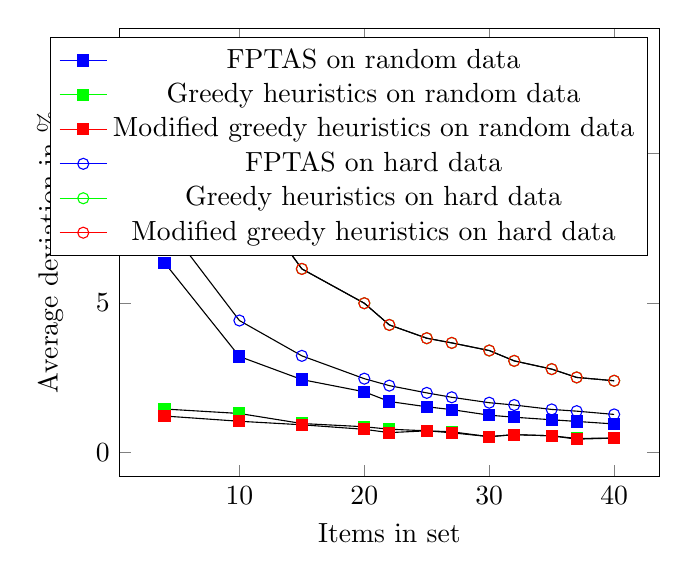
\begin{tikzpicture}
		\begin{axis}[
			xlabel=Items in set,
			ylabel=Average deviation in \%,
			scatter/classes={
				fptasN={mark=square*,blue},
				hungryN={mark=square*,green},
				singleN={mark=square*,red},
				fptasH={mark=o,blue},
				hungryH={mark=o,green},
				singleH={mark=o,red}
				}
			]
			\addplot[scatter,%
				scatter src=explicit symbolic]%
			table[meta=label] {
                x y label
                4 6.350120 fptasN
                10 3.210580 fptasN
                15 2.438080 fptasN
                20 2.029840 fptasN
                22 1.704882 fptasN
                25 1.528042 fptasN
                27 1.433396 fptasN
                30 1.247598 fptasN
                32 1.179112 fptasN
                35 1.093942 fptasN
                37 1.038356 fptasN
                40 .953716 fptasN
			};
			\addplot[scatter,%
				scatter src=explicit symbolic]%
			table[meta=label] {
				x y label
				4 1.453410 hungryN
                10 1.304166 hungryN
                15 .968396 hungryN
                20 .860422 hungryN
                22 .778518 hungryN
                25 .724522 hungryN
                27 .691782 hungryN
                30 .529006 hungryN
                32 .596280 hungryN
                35 .557696 hungryN
                37 .469084 hungryN
                40 .481640 hungryN
			};
			\addplot[scatter,%
				scatter src=explicit symbolic]%
			table[meta=label] {
                x y label
                4 1.219394 singleN
                10 1.043966 singleN
                15 .926256 singleN
                20 .774402 singleN
                22 .663398 singleN
                25 .724522 singleN
                27 .658822 singleN
                30 .529006 singleN
                32 .596280 singleN
                35 .557696 singleN
                37 .444584 singleN
                40 .481640 singleN
			};
			\addplot[scatter,%
				scatter src=explicit symbolic]%
			table[meta=label] {
				x y label
				4 7.711160 fptasH
                10 4.413000 fptasH
                15 3.231520 fptasH
                20 2.468120 fptasH
                22 2.235880 fptasH
                25 1.992836 fptasH
                27 1.845782 fptasH
                30 1.664936 fptasH
                32 1.586974 fptasH
                35 1.439758 fptasH
                37 1.382198 fptasH
                40 1.273106 fptasH
			};
			\addplot[scatter,%
				scatter src=explicit symbolic]%
			table[meta=label] {
				x y label
				4 12.939740 hungryH
                10 9.023060 hungryH
                15 6.139760 hungryH
                20 4.991380 hungryH
                22 4.266580 hungryH
                25 3.821660 hungryH
                27 3.664740 hungryH
                30 3.409840 hungryH
                32 3.063500 hungryH
                35 2.788140 hungryH
                37 2.510400 hungryH
                40 2.398320 hungryH
			};
			\addplot[scatter,%
				scatter src=explicit symbolic]%
			table[meta=label] {
                x y label
                4 12.430480 singleH
                10 9.023060 singleH
                15 6.139760 singleH
                20 4.991380 singleH
                22 4.266580 singleH
                25 3.821660 singleH
                27 3.664740 singleH
                30 3.409840 singleH
                32 3.063500 singleH
                35 2.788140 singleH
                37 2.510400 singleH
                40 2.398320 singleH
			};
			\addlegendentry{FPTAS on random data}
			\addlegendentry{Greedy heuristics on random data}
			\addlegendentry{Modified greedy heuristics on random data}
			\addlegendentry{FPTAS on hard data}
			\addlegendentry{Greedy heuristics on hard data}
			\addlegendentry{Modified greedy heuristics on hard data}
		\end{axis}
	\end{tikzpicture}
\caption{Average deviation in approximation algorithms}
\label{plot:deviation}
\end{figure}


% \begin{figure}
	\centering
	\pgfplotsset{every axis legend/.append style={
		at={(1.05,0.5)},
		anchor=west}}
	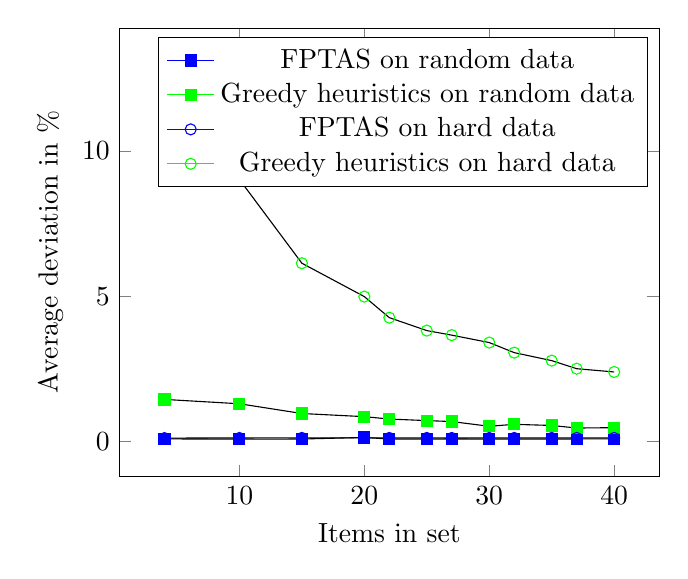
\begin{tikzpicture}
		\begin{axis}[
			xlabel=Items in set,
			ylabel=Average deviation in \%,
			scatter/classes={
				fptasN={mark=square*,blue},
				hungryN={mark=square*,green},
				fptasH={mark=o,blue},
				hungryH={mark=o,green}
				}
			]
			\addplot[scatter,%
				scatter src=explicit symbolic]%
			table[meta=label] {
                x y label
                4 .095931 fptasN
                10 .085455 fptasN
                15 .091002 fptasN
                20 .145440 fptasN
                22 .089912 fptasN
                25 .091948 fptasN
                27 .091139 fptasN
                30 .089941 fptasN
                32 .092691 fptasN
                35 .092870 fptasN
                37 .093395 fptasN
                40 .094362 fptasN
			};
			\addplot[scatter,%
				scatter src=explicit symbolic]%
			table[meta=label] {
				x y label
				4 1.453410 hungryN
                10 1.304166 hungryN
                15 .968396 hungryN
                20 .860422 hungryN
                22 .778518 hungryN
                25 .724522 hungryN
                27 .691782 hungryN
                30 .529006 hungryN
                32 .596280 hungryN
                35 .557696 hungryN
                37 .469084 hungryN
                40 .481640 hungryN
			};
			\addplot[scatter,%
				scatter src=explicit symbolic]%
			table[meta=label] {
				x y label
				4 .123029 fptasH
                10 .127224 fptasH
                15 .130156 fptasH
                20 .129032 fptasH
                22 .129395 fptasH
                25 .128979 fptasH
                27 .127454 fptasH
                30 .128554 fptasH
                32 .129028 fptasH
                35 .129171 fptasH
                37 .128856 fptasH
                40 .128841 fptasH
			};
			\addplot[scatter,%
				scatter src=explicit symbolic]%
			table[meta=label] {
				x y label
				4 12.939740 hungryH
                10 9.023060 hungryH
                15 6.139760 hungryH
                20 4.991380 hungryH
                22 4.266580 hungryH
                25 3.821660 hungryH
                27 3.664740 hungryH
                30 3.409840 hungryH
                32 3.063500 hungryH
                35 2.788140 hungryH
                37 2.510400 hungryH
                40 2.398320 hungryH
			};
			\addlegendentry{FPTAS on random data}
			\addlegendentry{Greedy heuristics on random data}
			\addlegendentry{FPTAS on hard data}
			\addlegendentry{Greedy heuristics on hard data}
		\end{axis}
	\end{tikzpicture}
\caption{Average deviation in FPTAS algorithm and greedy heuristics}
\label{plot:deviation1}
\end{figure}


% \begin{figure}
	\centering
	\pgfplotsset{every axis legend/.append style={
		at={(1.05,0.5)},
		anchor=west}}
	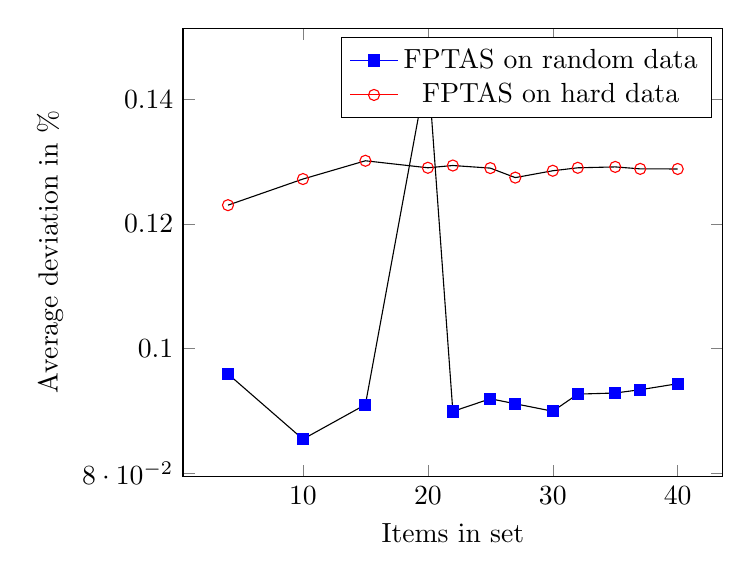
\begin{tikzpicture}
		\begin{axis}[
			xlabel=Items in set,
			ylabel=Average deviation in \%,
			scatter/classes={
				fptasN={mark=square*,blue},
				fptasH={mark=o,red}
				}
			]
			\addplot[scatter,%
				scatter src=explicit symbolic]%
			table[meta=label] {
                x y label
                4 .095931 fptasN
                10 .085455 fptasN
                15 .091002 fptasN
                20 .145440 fptasN
                22 .089912 fptasN
                25 .091948 fptasN
                27 .091139 fptasN
                30 .089941 fptasN
                32 .092691 fptasN
                35 .092870 fptasN
                37 .093395 fptasN
                40 .094362 fptasN
			};
			\addplot[scatter,%
				scatter src=explicit symbolic]%
			table[meta=label] {
				x y label
				4 .123029 fptasH
                10 .127224 fptasH
                15 .130156 fptasH
                20 .129032 fptasH
                22 .129395 fptasH
                25 .128979 fptasH
                27 .127454 fptasH
                30 .128554 fptasH
                32 .129028 fptasH
                35 .129171 fptasH
                37 .128856 fptasH
                40 .128841 fptasH
			};
			\addlegendentry{FPTAS on random data}
			\addlegendentry{FPTAS on hard data}
		\end{axis}
	\end{tikzpicture}
\caption{Average deviation in FPTAS algorithm}
\label{plot:deviation2}
\end{figure}



\section{Implementation}
All of these algorithms are implemented in Python 3.7, and all data were gathered on the Windows 10 OS running on Intel(R) Core(TM) i7-6700HQ CPU @ 2.60GHz.

For testing of these algorithms, we have used two data sets. The first one with randomly generated values and the second with purposefully hard data. However, in the randomly generated set, we can see a deviation in the dataset with twenty items. This deviation can be seen in \cref{plot:deviation,plot:maxDev,plot:devFptas}.


\subsection{Brute force algorithm}
The brute force algorithm is indifferent to any changes to a dataset by design, as it has to test every option before returning our solution, thus having the same average time complexity in all our test cases.

\subsection{Branch \& bounds algorithm}
As we observe the branch and bounds algorithm, we can see its relatively low complexity, which is mostly thanks to our data having considerably high knapsack with the 0.8 ratio between knapsacks load capacity and the combined weight of all the items. Thanks to this setup, the B\&B algorithm can skip a significant part of combinations, as it can add most of the elements. This difference can be observed in \cref{plot:fullTime}.

\subsection{Dynamic programing}
Our task was to use dynamic programming for solving the optimisation version of the 0/1 knapsack problem, for which we have selected the decomposition by value, due to its similarity with the FPTAS algorithm.

For more information about Dynamic programming or exact algorithm, feel free to look at the code attached or \cite[Moodle textbook]{WEBSITE:dynamicKnapsack}.

\subsection{Greedy heuristics}
The greedy algorithm sorts the elements given at input by the value to weight ratio. It adds as many elements as possible with the preference given to the items with the highest value and lowest weight.

This approach might not seem too precise, but it offers much lower complexity with $\mathbb{O}(n \log(n))$, where the most complex task is to sort the data.

\subsection{Modified greedy heuristics}
The modified greedy algorithm takes the maximum value item and compares it to the result of the basic greedy algorithm mentioned above. Afterwards, it takes the better of these results, which will be the result of our algorithm.

This algorithm allows us to approximate the result with the same complexity as the basic greedy heuristics, with a slight improvement in precision, as can be seen in \cref{plot:fptasTime}.

\subsection{FPTAS}

The FPTAS algorithm is basically the same as the decomposition by price used in dynamic programming.
The only difference here is that we lower the values of all the items, which lowers the complexity
of the algorithm and in this case, allows us to limit the imprecision.

In \cref{plot:fullTime,plot:deviation} we have set the highest deviation to be 0.5 and from 0.1 to 0.9 for \cref{plot:fptasTime,plot:devFptas}.
In order to gain precise data for selected maximal imprecisions, we have used the following formula.

\begin{itemize}
    \item $C_M = $max$\{c_1,c_2, ... c_n\}$
    \item $K = \dfrac{\epsilon C_M}{n}$
    \item $c_i' = \lfloor\dfrac{c_i}{K}\rfloor$
\end{itemize}

In \cref{plot:fptasTime,plot:devFptas} we can see the average time complexity and imprecision, respectively. From these graphs, we can clearly see the lowering time complexity with higher imprecision, as well as the lowering average imprecision, as the size of the set grows. 
% \begin{figure}
	\centering
	\pgfplotsset{every axis legend/.append style={
		at={(1.05,0.5)},
		anchor=west}}
	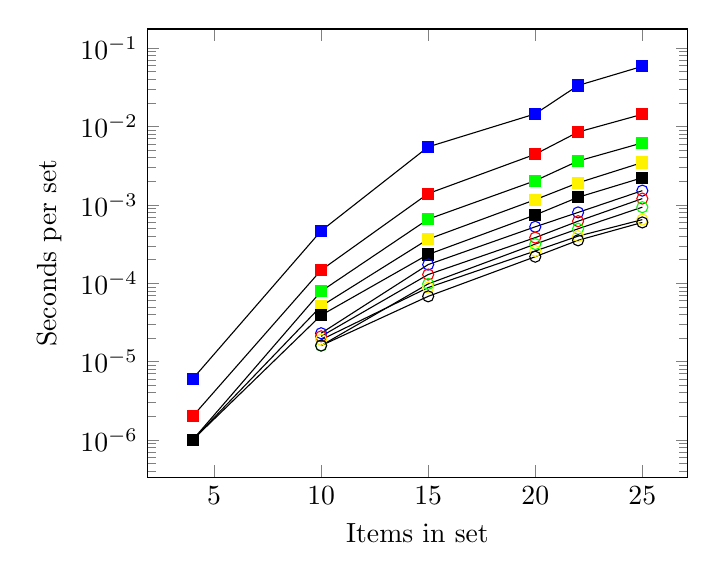
\begin{tikzpicture}
		\begin{semilogyaxis}[
			xlabel=Items in set,
			ylabel=Seconds per set,
			scatter/classes={
				fptas1={mark=square*,blue},
				fptas2={mark=square*,red},
				fptas3={mark=square*,green},
				fptas4={mark=square*,yellow},
				fptas5={mark=square*,black},
				fptas6={mark=o,blue},
				fptas7={mark=o,red},
				fptas8={mark=o,green},
				fptas9={mark=o,yellow},
				fptas10={mark=o,black},
				fptas11={mark=triangle*,blue},
				fptas12={mark=triangle*,red},
				fptas13={mark=triangle*,green},
				fptas14={mark=triangle*,yellow},
				fptas15={mark=triangle*,black},
				fptas16={mark=x,blue},
				fptas17={mark=x,red},
				fptas18={mark=x,green},
				fptas19={mark=x,yellow}
				}
			]
			\addplot[scatter,%
				scatter src=explicit symbolic]%
			table[meta=label] {
                x y label
                4 .000006 fptas1
                10 .000466 fptas1
                15 .005497 fptas1
                20 .014502 fptas1
                22 .033406 fptas1
                25 .058647 fptas1

			};
			\addplot[scatter,%
				scatter src=explicit symbolic]%
			table[meta=label] {
            x y label
            4 .000002 fptas2
            10 .000147 fptas2
            15 .001393 fptas2
            20 .004428 fptas2
            22 .008498 fptas2
            25 .014329 fptas2
			};
			\addplot[scatter,%
				scatter src=explicit symbolic]%
			table[meta=label] {
                x y label
4 .000001 fptas3
10 .000079 fptas3
15 .000657 fptas3
20 .002034 fptas3
22 .003628 fptas3
25 .006180 fptas3

			};
			\addplot[scatter,%
				scatter src=explicit symbolic]%
			table[meta=label] {
                x y label
4 .000001 fptas4
10 .000051 fptas4
15 .000365 fptas4
20 .001165 fptas4
22 .001910 fptas4
25 .003472 fptas4

			};
			\addplot[scatter,%
				scatter src=explicit symbolic]%
			table[meta=label] {
                x y label
4 .000001 fptas5
10 .000039 fptas5
15 .000233 fptas5
20 .000744 fptas5
22 .001250 fptas5
25 .002219 fptas5

			};
			\addplot[scatter,%
				scatter src=explicit symbolic]%
			table[meta=label] {x y label
            4 0 fptas6
            10 .000023 fptas6
            15 .000173 fptas6
            20 .000525 fptas6
            22 .000801 fptas6
            25 .001519 fptas6
			};
			\addplot[scatter,%
				scatter src=explicit symbolic]%
			table[meta=label] {x y label
            4 0 fptas7
            10 .000021 fptas7
            15 .000129 fptas7
            20 .000382 fptas7
            22 .000619 fptas7
            25 .001202 fptas7
            
			};
			\addplot[scatter,%
				scatter src=explicit symbolic]%
			table[meta=label] {x y label
            4 0 fptas8
            10 .000016 fptas8
            15 .000098 fptas8
            20 .000316 fptas8
            22 .000495 fptas8
            25 .000935 fptas8
            
			};
			\addplot[scatter,%
				scatter src=explicit symbolic]%
			table[meta=label] {x y label
            4 0 fptas9
            10 .000019 fptas9
            15 .000088 fptas9
            20 .000258 fptas9
            22 .000399 fptas9
            25 .000648 fptas9
            
			};
			\addplot[scatter,%
				scatter src=explicit symbolic]%
			table[meta=label] {x y label
            4 0 fptas10
            10 .000016 fptas10
            15 .000068 fptas10
            20 .000218 fptas10
            22 .000353 fptas10
            25 .000597 fptas10
            
			};
			% \addlegendentry{Dynamic price optimisation on random data}
			% \addlegendentry{FPTAS on random data}
			% \addlegendentry{Greedy heuristics on random data}
			% \addlegendentry{Single highest priced item on random data}
			% \addlegendentry{Dynamic price optimisation on hard data}
			% \addlegendentry{FPTAS on hard data}
			% \addlegendentry{Greedy heuristics on hard data}
			% \addlegendentry{Single highest priced item on hard data}
		\end{semilogyaxis}
	\end{tikzpicture}
\caption{Time needed depending on number of items in set}
\label{plot:fullTime}
\end{figure}

\begin{figure}
	\centering
	\pgfplotsset{every axis legend/.append style={
		at={(1.05,0.5)},
		anchor=west}}
	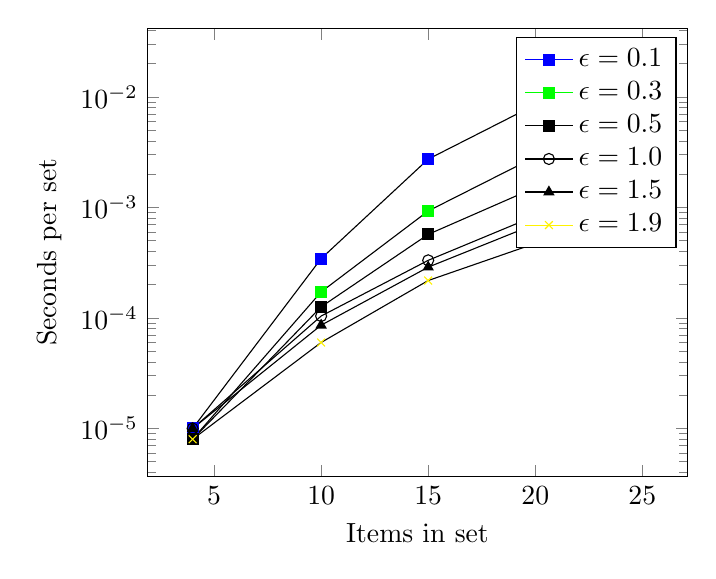
\begin{tikzpicture}
		\begin{semilogyaxis}[
			xlabel=Items in set,
			ylabel=Seconds per set,
			scatter/classes={
				fptas1={mark=square*,blue},
				% fptas2={mark=square*,red},
				fptas3={mark=square*,green},
				% fptas4={mark=square*,yellow},
				fptas5={mark=square*,black},
				% fptas6={mark=o,blue},
				% fptas7={mark=o,red},
				% fptas8={mark=o,green},
				% fptas9={mark=o,yellow},
				fptas10={mark=o,black},
				% fptas11={mark=triangle*,blue},
				% fptas12={mark=triangle*,red},
				% fptas13={mark=triangle*,green},
				% fptas14={mark=triangle*,yellow},
				fptas15={mark=triangle*,black},
				% fptas16={mark=x,blue},
				% fptas17={mark=x,red},
				% fptas18={mark=x,green},
				fptas19={mark=x,yellow}
				}
            ]
            
\addplot[scatter,scatter src=explicit symbolic]table[meta=label] {
x y label
4 .000010 fptas1
10 .000344 fptas1
15 .002732 fptas1
20 .008480 fptas1
22 .012136 fptas1
25 .019182 fptas1
};
\addplot[scatter,scatter src=explicit symbolic]table[meta=label] {
x y label
4 .000008 fptas3
10 .000172 fptas3
15 .000928 fptas3
20 .002864 fptas3
22 .003850 fptas3
25 .005866 fptas3
};
\addplot[scatter,scatter src=explicit symbolic]table[meta=label] {
x y label
4 .000008 fptas5
10 .000126 fptas5
15 .000570 fptas5
20 .001512 fptas5
22 .002132 fptas5
25 .003392 fptas5
};
\addplot[scatter,scatter src=explicit symbolic]table[meta=label] {
x y label
4 .000010 fptas10
10 .000104 fptas10
15 .000332 fptas10
20 .000838 fptas10
22 .001206 fptas10
25 .001826 fptas10
};
\addplot[scatter,scatter src=explicit symbolic]table[meta=label] {
x y label
4 .000010 fptas15
10 .000086 fptas15
15 .000288 fptas15
20 .000706 fptas15
22 .000966 fptas15
25 .001394 fptas15
};
\addplot[scatter,scatter src=explicit symbolic]table[meta=label] {
x y label
4 .000008 fptas19
10 .000060 fptas19
15 .000218 fptas19
20 .000472 fptas19
22 .000650 fptas19
25 .000842 fptas19
};

			\addlegendentry{$\epsilon = 0.1$}
			\addlegendentry{$\epsilon = 0.3$}
			\addlegendentry{$\epsilon = 0.5$}
			\addlegendentry{$\epsilon = 1.0$}
			\addlegendentry{$\epsilon = 1.5$}
			\addlegendentry{$\epsilon = 1.9$}
		\end{semilogyaxis}
	\end{tikzpicture}
\caption{Time needed depending on number of items in set}
\label{plot:fptasTime}
\end{figure}

\begin{figure}
	\centering
	\pgfplotsset{every axis legend/.append style={
		at={(1.05,0.5)},
		anchor=west}}
	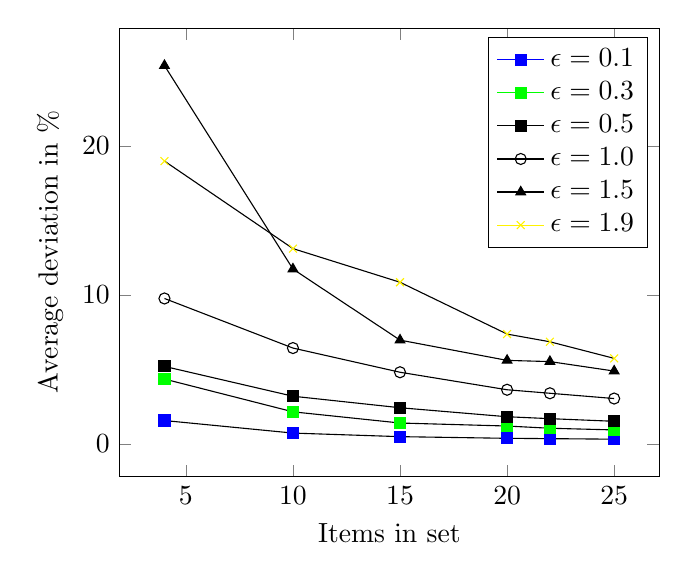
\begin{tikzpicture}
		\begin{axis}[
			xlabel=Items in set,
			ylabel=Average deviation in \%,
			scatter/classes={
				fptas1={mark=square*,blue},
				% fptas2={mark=square*,red},
				fptas3={mark=square*,green},
				% fptas4={mark=square*,yellow},
				fptas5={mark=square*,black},
				% fptas6={mark=o,blue},
				% fptas7={mark=o,red},
				% fptas8={mark=o,green},
				% fptas9={mark=o,yellow},
				fptas10={mark=o,black},
				% fptas11={mark=triangle*,blue},
				% fptas12={mark=triangle*,red},
				% fptas13={mark=triangle*,green},
				% fptas14={mark=triangle*,yellow},
				fptas15={mark=triangle*,black},
				% fptas16={mark=x,blue},
				% fptas17={mark=x,red},
				% fptas18={mark=x,green},
				fptas19={mark=x,yellow}
				}
            ]
            
\addplot[scatter,scatter src=explicit symbolic]table[meta=label] {
x y label
4 1.578520 fptas1
10 .736840 fptas1
15 .496943 fptas1
20 .385481 fptas1
22 .363280 fptas1
25 .327072 fptas1
};
\addplot[scatter,scatter src=explicit symbolic]table[meta=label] {
x y label
4 4.362344 fptas3
10 2.163470 fptas3
15 1.411930 fptas3
20 1.210040 fptas3
22 1.060910 fptas3
25 .949049 fptas3
};
\addplot[scatter,scatter src=explicit symbolic]table[meta=label] {
x y label
4 5.212682 fptas5
10 3.210590 fptas5
15 2.438080 fptas5
20 1.833507 fptas5
22 1.704880 fptas5
25 1.528040 fptas5
};
\addplot[scatter,scatter src=explicit symbolic]table[meta=label] {
x y label
4 9.771065 fptas10
10 6.443160 fptas10
15 4.819690 fptas10
20 3.644278 fptas10
22 3.408830 fptas10
25 3.055040 fptas10
};
\addplot[scatter,scatter src=explicit symbolic]table[meta=label] {
x y label
4 25.401756 fptas15
10 11.745500 fptas15
15 6.976230 fptas15
20 5.615681 fptas15
22 5.535220 fptas15
25 4.898940 fptas15
};
\addplot[scatter,scatter src=explicit symbolic]table[meta=label] {
x y label
4 18.992468 fptas19
10 13.119000 fptas19
15 10.859700 fptas19
20 7.381382 fptas19
22 6.864850 fptas19
25 5.750920 fptas19
};

			\addlegendentry{$\epsilon = 0.1$}
			\addlegendentry{$\epsilon = 0.3$}
			\addlegendentry{$\epsilon = 0.5$}
			\addlegendentry{$\epsilon = 1.0$}
			\addlegendentry{$\epsilon = 1.5$}
			\addlegendentry{$\epsilon = 1.9$}
		\end{axis}
	\end{tikzpicture}
\caption{Average deviation depending on number of items in set}
\label{plot:devFptas}
\end{figure}

\begin{figure}
	\centering
	\pgfplotsset{every axis legend/.append style={
		at={(1.05,0.5)},
		anchor=west}}
	\begin{tikzpicture}
		\begin{axis}[
			xlabel=Items in set,
			ylabel=Highest deviation in \%,
			scatter/classes={
				fptas1={mark=square*,blue},
				fptas3={mark=square*,green},
				fptas5={mark=square*,black},
				fptas7={mark=square*,red},
				fptas9={mark=square*,yellow}
				}
            ]
            

			\addlegendentry{$\epsilon = 0.1$}
			\addlegendentry{$\epsilon = 0.3$}
			\addlegendentry{$\epsilon = 0.5$}
			\addlegendentry{$\epsilon = 0.7$}
			\addlegendentry{$\epsilon = 0.9$}
		\end{axis}
	\end{tikzpicture}
\caption{Highest deviation for each set of items}
\label{plot:maxDev}
\end{figure}

\begin{figure}
	\centering
	\pgfplotsset{every axis legend/.append style={
		at={(1.05,0.5)},
		anchor=west}}
	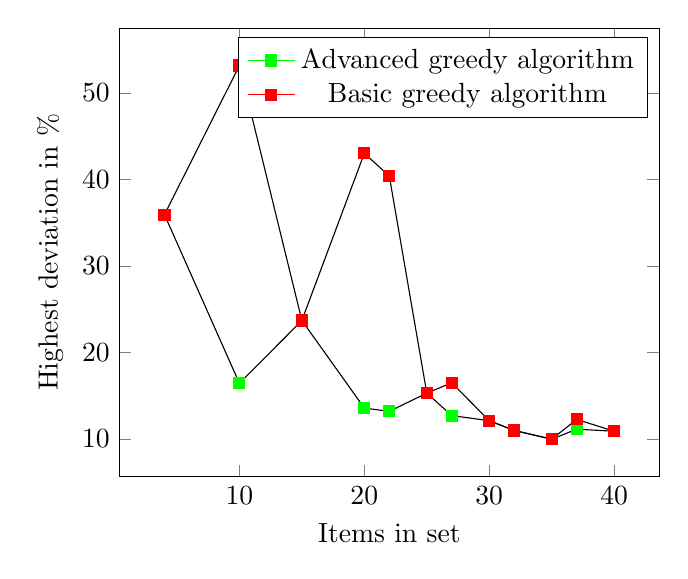
\begin{tikzpicture}
		\begin{axis}[
			xlabel=Items in set,
			ylabel=Highest deviation in \%,
			scatter/classes={
				% fptas1={mark=square*,blue},
				advancedGreedy1={mark=square*,green},
				solveHungry1={mark=square*,red}
				}
            ]
% \addplot[scatter,scatter src=explicit symbolic]table[meta=label] {
% x y label
% 4 0.0835 fptas1
% 10 0.009412 fptas1
% 15 0.005128 fptas1
% 20 0.0019934 fptas1
% 22 0.002894 fptas1
% 25 0.002714 fptas1
% };
\addplot[scatter,scatter src=explicit symbolic]table[meta=label] {
x y label
4 35.92 advancedGreedy1
10 16.42 advancedGreedy1
15 23.68 advancedGreedy1
20 13.56 advancedGreedy1
22 13.18 advancedGreedy1
25 15.29 advancedGreedy1
27 12.69 advancedGreedy1
30 12.1 advancedGreedy1
32 10.97 advancedGreedy1
35 9.964 advancedGreedy1
37 11.12 advancedGreedy1
40 10.88 advancedGreedy1
};
\addplot[scatter,scatter src=explicit symbolic]table[meta=label] {
x y label
4 35.92 solveHungry1
10 53.15 solveHungry1
15 23.68 solveHungry1
20 43.01 solveHungry1
22 40.38 solveHungry1
25 15.29 solveHungry1
27 16.48 solveHungry1
30 12.1 solveHungry1
32 10.97 solveHungry1
35 9.964 solveHungry1
37 12.25 solveHungry1
40 10.88 solveHungry1
};
			% \addlegendentry{FPTAS algorithm with $\epsilon = 0.1$}
			\addlegendentry{Advanced greedy algorithm}
			\addlegendentry{Basic greedy algorithm}
		\end{axis}
	\end{tikzpicture}
\caption{Highest deviation in greedy algorithms for each set of items on normal dataset}
\label{plot:maxDev}
\end{figure}


\newpage

\section{Conclusion}
In conclusion, we have created six implementations for solving the optimisation version of the 0/1 knapsack problem. We have compared the efficiency of these implementations with respect to processor time and their precision. This comparison was made on randomly generated data set as well as on a purposefully hard dataset. However, the difference between those two datasets did not appear to be particularly apparent, which might have been caused by the concrete implementation.

Furthermore,  we have also compared the time complexity and the imprecision within the FPTAS algorithm for multiple maximal imprecisions. From these, we have selected few to show in \cref{plot:fptasTime,plot:devFptas}.

\newpage
\bibliographystyle{iso690}
\nocite{*} % all entries in the bib file
\bibliography{database.bib}

\end{document}